% =====================================================================
%  ISDS 2026 -- The 4th International Conference on Intelligent Systems
%  and Data Science, Yuan Ze University, Taiwan, 14-15 November 2026
%
%  COMPACT long-paper variant, trimmed to the 12-15 page limit.
%  Format: Springer LNCS/CCIS one-column (llncs.cls), English, PDF.
%  Track 3 -- Image Processing & Pattern Recognition
%  Submission: https://easychair.org/conferences/?conf=isds2026
%
%  Trimmed relative to ISDS2026_FGSS.tex (see ISDS2026_SUBMISSION_CHECK.md):
%    - 12 figures -> 5   (kept: architecture, qualitative grid, frequency
%      decomposition, robustness overview, training curve)
%    - 11 tables  -> 6   (dropped: relwork positioning, loss cheat-sheet,
%      cross-family SOTA context, inference budget -> moved to prose;
%      serial-2 and serial-3 merged into one table, blend_* rows dropped;
%      ablation table also folded into prose to meet the 12-15 page limit)
%    - Introduction 6 -> 3 paragraphs; reverse-decoder / reverse-loss and
%      protocol / implementation subsections condensed; loss hyper-parameter
%      list moved to a footnote
%  Build: pdflatex ISDS2026_FGSS_compact (x2)
% =====================================================================
\documentclass[runningheads]{llncs}
\setlength{\paperwidth}{210mm}
\setlength{\paperheight}{297mm}
\pdfpagewidth=\paperwidth
\pdfpageheight=\paperheight

\usepackage{cmap}
\usepackage[T1]{fontenc}
\usepackage[utf8]{inputenc}
\usepackage{lmodern}
\usepackage{amsmath,amssymb,amsfonts}
\usepackage{graphicx}
\usepackage{textcomp}
\usepackage[table]{xcolor}
\newcommand{\revised}[1]{\textcolor{blue}{#1}}
\usepackage{booktabs}
\usepackage{multirow}
\usepackage{array}
\usepackage{url}
\usepackage{float}
\usepackage{colortbl}
\usepackage{algorithm}
\usepackage{algpseudocode}
\usepackage{placeins}

\usepackage[hidelinks]{hyperref}
\providecommand{\doi}[1]{\href{https://doi.org/#1}{https://doi.org/#1}}

\renewcommand{\arraystretch}{1.0}
\setlength{\tabcolsep}{4pt}
\definecolor{rowshade}{HTML}{F2F2F2}

\renewcommand{\topfraction}{0.85}
\renewcommand{\bottomfraction}{0.70}
\renewcommand{\dbltopfraction}{0.85}
\renewcommand{\textfraction}{0.10}
\renewcommand{\floatpagefraction}{0.75}
\renewcommand{\dblfloatpagefraction}{0.75}

\begin{document}

\title{Frequency-Guided Semantic Steganography for High-Fidelity Self-Contained Style-Transfer Image Hiding}

\titlerunning{Frequency-Guided Semantic Steganography}

\author{%
Ngoc-Giau Pham\inst{1,2} \and
Minh-Tuan Bui\inst{3} \and
Phuoc-Hung Vo\inst{1}\textsuperscript{(\textrm{*})}%
}

\authorrunning{N.-G. Pham et al.}

\institute{%
College of Engineering and Technology, Tra Vinh University, Vinh Long, Vietnam\\
\email{hungvo@tvu.edu.vn}
\and
Faculty of Engineering and Technology, Tien Giang University, Dong Thap, Vietnam\\
\email{phamngocgiau@tgu.edu.vn}
\and
RMIT University, Ho Chi Minh City, Vietnam\\
\email{bmtuan0704@gmail.com}\\[2pt]
\textsuperscript{(\textrm{*})}\,Corresponding author
}

\maketitle

\begin{abstract}
% SOURCE: run_summary.json, paper_table_main.csv, token_summary.csv, ablation.csv, robustness_metrics.csv
Style-transfer steganography uses the texture of stylised images to mask embedding residuals, but repeated stylisation can degrade recovery. We investigate two design choices that contribute to this trade-off: distortion regularisers without a target-fidelity threshold and spatially dense payloads. FGSS encodes the secret as a $\mathbf{z}\!\in\!\mathbb{R}^{64\times32\times32}$ semantic token and an auxiliary thumbnail. It applies a target-calibrated penalty above an MSE threshold derived from a desired cover PSNR, together with a wavelet-inspired term that discourages low-frequency residual energy. An oracle-guided reverse decoder and probabilistic future-pass supervision train the model for recovery after as many as three cumulative stylisation passes. On $600$ COCO val2017 content--style pairs, FGSS obtains $39.61\pm0.35$\,dB cover PSNR, $0.9914$ SSIM, and $0.0195$ LPIPS. Clean-channel reverse SSIM rises from $0.5234$ for the content-free baseline to $0.8070$ with the decoded token; an oracle-token diagnostic reaches $0.8136$. In a reduced $192\!\times\!192$ single-pair ablation, the target-calibrated penalty increases cover PSNR by $5.76$\,dB. Token MSE differs by at most $1.2\!\times\!10^{-4}$ across the integrated clean, Gaussian, and JPEG-style channels. The embedding path has $1.9$\,M parameters and runs in $0.0096$\,s per image on an RTX~5070~Ti. \revised{Pretrained checkpoints, code, and split manifests are publicly available for full reproducibility.\footnote{\revised{Code and checkpoints repository: \url{https://github.com/phamngocgiau/FGSS-ISDS2026}}}}

\keywords{Image steganography \and Neural style transfer \and Frequency-domain learning \and Capacity ceiling \and Robustness \and Semantic tokens.}
\end{abstract}

\section{Introduction}

Deep image-hiding models can carry larger payloads than traditional least-significant-bit methods, but their residuals may remain detectable by learned steganalysers~\cite{isn,riis,rmsteg}. Style-transfer steganography instead uses the naturally variable texture of a stylised carrier~\cite{wacv2020,stylestegan2023,sstegogan2024,sst2024,ihst2024,css2024,sddpm2025,stisgan2026}. In the self-contained setting~\cite{wacv2020}, the receiver reconstructs the original content from the stego image and shared model weights. Published methods still show a marked trade-off between cover fidelity and recovery, particularly after a second or third stylisation pass~\cite{wacv2020,stylestegan2023}.

We study two choices in this trade-off: a coefficient-weighted distortion loss with no target-fidelity threshold, and a payload that spans the carrier spatially. FGSS replaces the spatial secret with a fixed-size semantic token and thumbnail. Its capacity-ceiling loss is a soft, one-sided penalty above an MSE threshold computed from a target PSNR; a separate low/high-frequency proxy discourages residual energy in the low-frequency band. Oracle-guided reverse decoding and serial-consistency supervision are used to improve recovery after repeated transformations.

% SOURCE: run_summary.json (cover_metrics_mean), token_summary.csv, ablation.csv
The full model has $10.7$\,M parameters, of which $1.9$\,M are used on the embedding path. On $600$ COCO val2017~\cite{coco} pairs, it obtains $39.61$\,dB cover PSNR, $0.9914$ SSIM~\cite{ssim}, and $0.0195$ LPIPS~\cite{lpips}. The contributions are: (i) a target-calibrated soft penalty on cover MSE; (ii) a differentiable frequency proxy that penalises low-frequency residual energy; (iii) a compact semantic-token payload; and (iv) reverse and serial-recovery experiments, including robustness and steganalysis probes. The reduced single-pair ablation changes cover PSNR from $35.61$ to $41.37$\,dB when the target-calibrated penalty is enabled.

\section{Related Work}
\label{sec:relwork}

\subsection{Deep Image-in-Image Steganography}
Recent image-hiding systems use invertible networks~\cite{isn}, normalising flows~\cite{riis}, attention modules~\cite{rmsteg}, and frequency-domain objectives~\cite{rfs2023}. These models can carry full images or message grids, although learned detectors such as SRNet~\cite{srnet} and XuNet~\cite{xunet} may still identify residual statistics. FGSS does not claim undetectability; it uses a target-calibrated distortion penalty and reports detector results in Section~\ref{sec:sota}.

\subsection{Coverless and Generative Steganography}
Coverless steganography and steganography without embedding generate or select containers through disentanglement models~\cite{ideas2022,siswe2023} or diffusion models~\cite{cross}. Because these approaches do not add a conventional embedding residual, their payload definition and carrier control differ from residual-based image hiding. FGSS adopts a compact latent payload but retains a deterministic style-transfer carrier and a bounded-scale residual.

\subsection{Style Transfer Steganography}
Style-transfer steganography hides information in, or alongside, features used for artistic stylisation~\cite{wacv2020,quat2021,stylestegan2023,sstegogan2024,sst2024,sddpm2025,stisgan2026}. Existing systems use different carriers, payloads, and fidelity targets, which makes direct PSNR comparison difficult. FGSS adds an explicit target-derived MSE threshold to the training objective; the threshold is a soft penalty rather than a hard guarantee on test images.

\begin{figure}[!t]
    \centering
    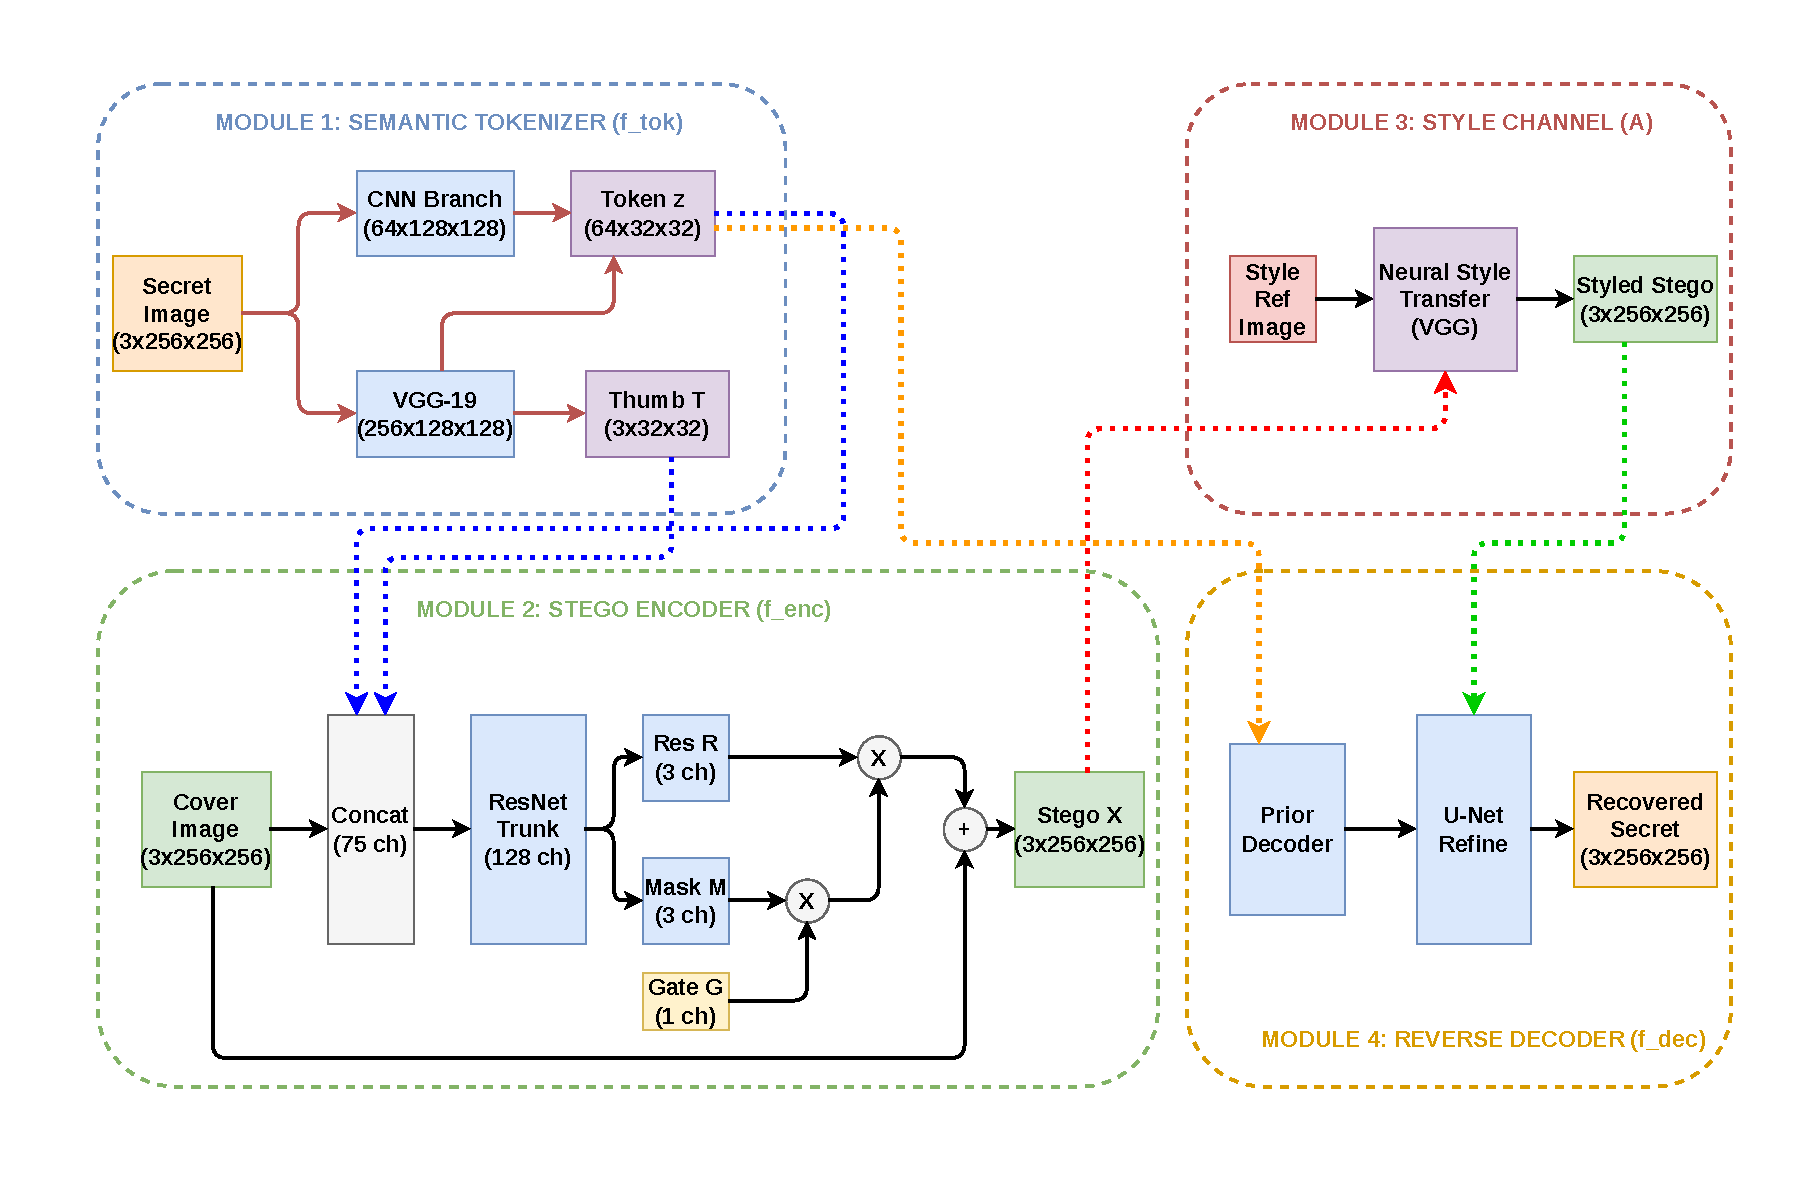
\includegraphics[width=\textwidth]{paper_assets/architecture_diagram.pdf}
    \caption{Master architectural overview of the proposed Frequency-Guided Semantic Steganography (FGSS) framework. The diagram illustrates the data flow across four distinct modules enclosed in dashed bounding frames: (i) Module 1: Semantic Tokenizer $f_{\text{tok}}$; (ii) Module 2: Stego Encoder $f_{\text{enc}}$ with capacity ceiling \& texture gate $\mathbf{G}$; (iii) Module 3: Style Transfer \& Attack Channel $\mathcal{A}$; and (iv) Module 4: Reverse Decoder $f_{\text{rev}}$ with oracle distillation. Feature map dimensions ($C \times H \times W$) are denoted within each functional block.}
    \label{fig:architecture}
\end{figure}

\section{Proposed Method}
\label{sec:method}

\subsection{Notation and System Overview}
Scalars are plain math italic, vectors bold lower case, tensors bold upper case. The cover image is $\mathbf{X}_{\text{cover}}\!\in\!\mathbb{R}^{3\times H\times W}$, the secret content is $\mathbf{C}\!\in\!\mathbb{R}^{3\times H\times W}$ and the painting reference is $\mathbf{S}$. The cover is obtained by an optimisation-based stylisation operator $f_{\text{style}}(\mathbf{C},\mathbf{S})$ held fixed during stego training. We write $\mathbf{z}\!\in\!\mathbb{R}^{d_{\text{tok}}\times g_{\text{tok}}\times g_{\text{tok}}}$ for the semantic token used as payload and $\mathbf{T}\!\in\!\mathbb{R}^{3\times g_{\text{tok}}\times g_{\text{tok}}}$ for the auxiliary thumbnail, with $g_{\text{tok}}=32$ and $d_{\text{tok}}=64$ throughout; because the tokenizer ends in an adaptive pooling stage, the same token geometry is produced at both the $256\!\times\!256$ benchmark resolution and the $192\!\times\!192$ CPU resolution.

The system consists of four learnable modules --- a semantic tokenizer $f_{\text{tok}}$, a stego encoder $f_{\text{enc}}$, a stego decoder $f_{\text{dec}}$ and a reverse decoder $f_{\text{rev}}$ --- together with a non-learnable attack channel $\mathcal{A}$. All four are trained jointly; Figure~\ref{fig:architecture} summarises the data flow. Training and inference share the same flow. The channel is enumerated over its three modes in both regimes: during training so the decoder sees clean and degraded inputs in a balanced fashion, and at evaluation so every pair is scored under each mode separately.


\subsection{Cover Generation}
\label{sec:cover}
The cover is computed deterministically from $(\mathbf{C},\mathbf{S})$ by an optimisation-based operator $f_{\text{style}}$ in the spirit of Gatys~\cite{gatys}: a target image initialised at $\mathbf{C}$ is optimised for $T_{\text{nst}}$ steps with Adam~\cite{adam}, learning rate $0.03$, content weight $1.0$ on the \texttt{conv\_3} feature map of an ImageNet-pretrained VGG-19~\cite{vgg}, and style weight $6\!\times\!10^{5}$ on the Gram matrices of \texttt{conv\_1}--\texttt{conv\_5}. We use $T_{\text{nst}}\!=\!45$ for the $256\!\times\!256$ benchmark and $T_{\text{nst}}\!=\!120$ for the $192\!\times\!192$ CPU smoke run. $f_{\text{style}}$ is frozen throughout stego training and its outputs are cached per $(\mathbf{C},\mathbf{S})$ pair to keep the inner loop deterministic.



\subsection{Semantic Tokenisation of the Secret}
\label{sec:tok}
Spatially extended payloads require the encoder to distribute changes over many carrier locations. We reduce this footprint by representing the secret with a fixed-size latent token. The tokenizer $f_{\text{tok}}$ has two branches. Its CNN branch contains three stride-two $\text{Conv}_{3{\times}3}{+}\text{GroupNorm}{+}\text{GELU}$~\cite{gelu} blocks, two residual blocks, and a $1\!\times\!1$ projection to $d_{\text{tok}}$ channels, followed by adaptive pooling to $g_{\text{tok}}\!\times\!g_{\text{tok}}$. The VGG branch extracts the \texttt{conv\_3} feature map from a frozen VGG-19~\cite{vgg}, projects it through two $1\!\times\!1$ convolutions ($256 \!\to\! h \!\to\! d_{\text{tok}}$), and applies the same pooling. We use $h=128$. The two outputs are summed and passed through a hyperbolic tangent:
\begin{equation}
    \mathbf{z} = \tanh\!\left(\mathbf{z}_{\text{cnn}} + \mathbf{z}_{\text{vgg}}\right).
    \label{eq:tok}
\end{equation}
In parallel, a ConvBlock, residual block, and $1\!\times\!1$ head refine a bilinearly resized RGB thumbnail $\mathbf{T}$. The payload $(\mathbf{z},\mathbf{T})$ contains $68\,608$ values, compared with $196\,608$ values in a $3\!\times\!256\!\times\!256$ image. This is a lossy latent representation, not a raw message bitstream: it serialises to $33.5$\,bpp in FP32 or $8.375$\,bpp as \texttt{uint8} relative to a $256\!\times\!256$ carrier. The receiver also needs the trained decoder weights. FGSS therefore targets self-contained stylisation with a shared model rather than keyless bitstream steganography.

\subsection{Stego Encoder and Decoder Architecture}
\label{sec:enc}
The encoder concatenates the cover with four auxiliary feature maps: the up-sampled token, the up-sampled thumbnail, a two-channel Sobel map, and the cover--thumbnail difference. We denote the last two maps by $\mathbf{E}$ and $\mathbf{D}$. Together the inputs have $75$ channels. A ConvBlock$(75\!\to\!h)$ stem and three ResidualBlocks$(h)$ feed a residual head $\mathbf{R}=\tanh(\text{Conv}_{3\times3}(\cdot))$ and a mask head $\mathbf{M}_{\text{learned}}=\sigma(\text{Conv}_{3\times3}(\cdot))$. The mask is modulated by a detached texture gate $\mathbf{G}$ computed from the mean absolute Sobel response and half the mean magnitude of the three high-frequency Haar sub-bands. The gate is normalised per image, clamped to $[0,1]$, and given a floor $\tau_{\text{floor}}=0.6$:
\begin{align}
    \mathbf{M} &= \mathbf{M}_{\text{learned}} \odot \left[\tau_{\text{floor}} + (1-\tau_{\text{floor}})\,\mathbf{G}\right], \label{eq:mask}\\
    \mathbf{X}_{\text{stego}} &= \mathrm{clip}_{[0,1]}\!\left(\mathbf{X}_{\text{cover}}+\alpha\,\sigma\,\mathbf{M}\odot\mathbf{R}\right),
    \label{eq:stego}
\end{align}
where $\alpha\!=\!0.025$ is a fixed residual scale and $\sigma\!\in\![1.02,1.30]$ at training ($\sigma_{\text{eval}}\!=\!1.24$). Masking steers perturbation energy towards textured regions and away from flat, perceptually salient areas, directly complementing the frequency loss. The trunk width is $h\!=\!128$ at both evaluation resolutions.



The decoder $f_{\text{dec}}$ is the dual of the tokenizer-plus-encoder: it consumes a $3\!\times\!H\!\times\!W$ stego image, applies three strided ConvBlocks and one ResStack, adaptively pools to $g_{\text{tok}}\!\times\!g_{\text{tok}}$, and projects with $1\!\times\!1$ convolutions to $\hat{\mathbf{z}}$ and to a sigmoidal thumbnail $\hat{\mathbf{T}}$ used as a reconstruction anchor. We use a single decoder rather than one per attack mode, for simplicity and to encourage representation transfer across distortion types.

\subsection{Attack Channel and Strength Curriculum}
\label{sec:attack}
The decoder is supervised under three modes of an attack channel $\mathcal{A}$:
\begin{align*}
    \mathcal{A}_{\text{id}}(\mathbf{X}) &= \mathbf{X}, \\
    \mathcal{A}_{\text{jpeg}}(\mathbf{X}) &= q\mathbf{X}+(1-q)\,\mathrm{AvgPool}_{3,1}(\mathbf{X}),\quad q=0.65, \\
    \mathcal{A}_{\text{rbn}}(\mathbf{X}) &= \mathrm{clip}_{[0,1]}(\mathbf{X}+\sigma_{n}\boldsymbol{\xi}),\quad \boldsymbol{\xi}\!\sim\!\mathcal{N}(0,I),\ \sigma_{n}=0.02.
\end{align*}
The JPEG-style proxy mimics the low-pass tendency of moderately compressed JPEGs without breaking gradient flow; the Gaussian mode adds zero-mean noise. \revised{This differentiable proxy $\mathcal{A}_{\text{jpeg}}$ is employed strictly for backpropagation during training; test-time robustness is subsequently evaluated under real DCT JPEG compression (Section~\ref{sec:exp_coco}) along with noise and geometric transformations.} The strength scalar $\sigma_{\text{train}}$ is sampled per minibatch from $[1.02,1.30]$ to expose the decoder to a range of embedding magnitudes. All reported test-time results use the fixed value $\sigma_{\text{eval}}=1.24$, near the upper end of that range. During training we additionally monitor a held-out partition at a slightly stronger $\sigma=1.36$ for checkpoint selection, so the selected model is chosen under a marginally harder condition than the one it is finally reported at.

\subsection{Frequency-Guided Embedding Strategy}
\label{sec:freq}
A standard pixelwise cover loss penalises all spatial frequencies equally. FGSS instead separates a low-frequency proxy from the remaining residual:
\begin{align}
    \boldsymbol{\Delta} &= \mathbf{X}_{\text{stego}}-\mathbf{X}_{\text{cover}}, \label{eq:residual_def} \\
    \boldsymbol{\Delta}_{\text{LL}} &= \mathcal{U}\!\left(\mathcal{P}_{2,2}(\boldsymbol{\Delta})\right), \quad
    \boldsymbol{\Delta}_{\text{HH}} = \boldsymbol{\Delta}-\boldsymbol{\Delta}_{\text{LL}},
\end{align}
where $\mathcal{P}_{2,2}$ is a $2\!\times\!2$ average-pooling operator with stride two and $\mathcal{U}$ a bilinear up-sampler back to the original resolution. The pair $(\mathcal{P}_{2,2},\mathcal{U})$ is a differentiable, parameter-free proxy for the $LL$ band of a one-level Haar discrete wavelet transform. We use the proxy rather than an exact DWT here because it returns the low band already resampled to the input resolution, so the residual split needs no interpolation bookkeeping; an exact Haar transform is used separately for the texture gate of Section~\ref{sec:enc}, where the high sub-bands are needed individually. The frequency loss is
\begin{equation}
    \mathcal{L}_{\text{freq}} = \text{MSE}\!\left(\boldsymbol{\Delta}_{\text{LL}}\right) - \lambda_{\text{HH}}\,\text{MSE}\!\left(\boldsymbol{\Delta}_{\text{HH}}\right),
    \label{eq:freq}
\end{equation}
with $\lambda_{\text{HH}}\!=\!0.1$. The first term penalises perturbations in the low-frequency band carrying colour and structure; the second is a small \emph{negative} term that explicitly rewards placing energy in the high-frequency band, where the human visual system is least sensitive. We weight $\mathcal{L}_{\text{freq}}$ by $\lambda_{\text{dwt}}\!=\!0.2$ in the joint objective. \revised{Because the Haar wavelet decomposition is orthonormal and energy-preserving ($\|\boldsymbol{\Delta}\|_2^2 = \sum_b \|\boldsymbol{\Delta}_b\|_2^2$), aggregate cover PSNR depends strictly on total residual MSE rather than subband allocation. The objective $\mathcal{L}_{\text{freq}}$ penalises smooth carrier perturbations ($\boldsymbol{\Delta}_{\text{LL}}$) while rewarding high-frequency placement ($\boldsymbol{\Delta}_{\text{HH}}$) where human visual contrast sensitivity is lowest. Disabling $\mathcal{L}_{\text{freq}}$ thus leaves aggregate cover PSNR unchanged at the reported precision ($41.37$\,dB) by Parseval conservation, while steering energy away from low frequencies suppresses visual mottling, directly supporting low perceptual distortion ($\text{LPIPS}=0.0195$).} In addition, three coarse band-statistics of the residual are supervised against a smooth target shape derived from the texture mask $\mathbf{M}$:
\begin{equation}
\begin{aligned}
    \mathcal{L}_{\text{embed}} = & \,\lambda_{\text{em-l}}\!\left\|\mathrm{LP}(\boldsymbol{\Delta})\right\|_1
    + \lambda_{\text{em-t}}\!\left\|(1-\mathbf{M})\odot\boldsymbol{\Delta}\right\|_1 \\
    & + \lambda_{\text{em-h}}\!\left\|\boldsymbol{\Delta}-\mathrm{LP}(\boldsymbol{\Delta})\right\|_1,
\end{aligned}
    \label{eq:embed}
\end{equation}
with $(\lambda_{\text{em-l}},\lambda_{\text{em-t}},\lambda_{\text{em-h}})=(0.5,0.3,0.12)$ and $\mathrm{LP}=\mathcal{U}\circ\mathcal{P}_{2,2}$. The first term suppresses low-frequency leakage, the second penalises perturbation outside textured regions, and the third lightly regulates the high band so it does not become arbitrarily noisy.

\subsection{Nonlinear Capacity-Ceiling Penalty}
\label{sec:ceil}
For images scaled to $[0,1]$, a target cover PSNR $\tau_{\text{psnr}}$ corresponds to the MSE threshold $\epsilon = 10^{-\tau_{\text{psnr}}/10}$. For example, $\tau_{\text{psnr}}\!\approx\!39$\,dB gives $\epsilon\!\approx\!1.2\!\times\!10^{-4}$. We define the capacity-ceiling loss as
\begin{equation}
    \mathcal{L}_{\text{cap}} = \lambda_{\text{cov}}\,\text{MSE}(\boldsymbol{\Delta}) + \lambda_{\text{ceil}} \left(\frac{\max\!\left(0,\text{MSE}(\boldsymbol{\Delta})-\epsilon\right)}{\epsilon}\right)^{\!2},
    \label{eq:cap}
\end{equation}
with $\lambda_{\text{cov}}\!=\!25$ and $\lambda_{\text{ceil}}\!=\!30$. The second term is a one-sided quadratic penalty that activates when empirical cover MSE exceeds $\epsilon$. Normalising the excess by $\epsilon$ makes the penalty dimensionless. This is a soft training constraint: it discourages, but does not mathematically prevent, test-time MSE above the threshold. We also use $\mathcal{L}_{\text{prior}}=\|\mathbf{R}\|_2^2$ (weight $4.5$) and a Gram-matrix style-retention term $\mathcal{L}_{\text{style-cov}}$ (weight $0.06$).

\subsection{Reverse Decoder, Oracle Distillation and Serial Consistency}
\label{sec:rev}
The reverse decoder $f_{\text{rev}}$ reconstructs the original content $\mathbf{C}$ from the decoded token $\hat{\mathbf{z}}$ and thumbnail $\hat{\mathbf{T}}$ using two cascaded sub-networks. A \emph{Token Prior Decoder} progressively up-samples the concatenation $(\hat{\mathbf{z}},\hat{\mathbf{T}})$ through three stages, each a ConvBlock followed by a ResidualBlock, doubling the spatial resolution at every stage ($32\!\to\!64\!\to\!128\!\to\!256$), producing a coarse prior $\mathbf{P}\!\in\!\mathbb{R}^{3\times H\times W}$ and intermediate maps $\{\mathbf{f}_{128},\mathbf{f}_{256}\}$. A \emph{U-Net refinement decoder} then fuses the stego image with the prior; its $80$-channel input concatenates the stego image, the prior, the up-sampled thumbnail and token, Sobel edges of both stego and prior, and their absolute difference. The U-Net has two stride-2 encoder stages, a two-block bottleneck, and two decoder stages whose skip connections also incorporate $\mathbf{f}_{128}$ and $\mathbf{f}_{256}$. Two heads produce a blend map $\boldsymbol{\beta}=\sigma(\text{Conv}_{3\times3}(\cdot))$ and a delta $\boldsymbol{\delta}=\tanh(\text{Conv}_{3\times3}(\cdot))$:
\begin{equation}
    \hat{\mathbf{C}} = \mathrm{clip}_{[0,1]}\!\Big(\boldsymbol{\beta}\odot\mathbf{P} + (1{-}\boldsymbol{\beta})\odot\mathrm{up}(\hat{\mathbf{T}}) + \gamma\,\boldsymbol{\delta}\Big),
    \label{eq:revdec}
\end{equation}
with $\gamma\!=\!0.22$; the network therefore combines a learned prior, the thumbnail, and a residual correction.



The reverse loss combines three attack-conditioned terms, $\mathcal{L}_{\text{rev}} = \lambda_{\text{r}}\mathcal{L}_{\text{rev,id}} + \lambda_{\text{rR}}\mathcal{L}_{\text{rev,rbn}} + \lambda_{\text{rJ}}\mathcal{L}_{\text{rev,jpeg}}$ with $(\lambda_{\text{r}},\lambda_{\text{rR}},\lambda_{\text{rJ}})=(25,12,12)$. Each term includes Charbonnier, VGG-feature, edge, low-frequency, Fourier-magnitude and colour-mean losses, plus a content--cover margin in feature space. For oracle distillation, the reverse decoder is also evaluated with the detached ground-truth token and thumbnail to produce a reference $\hat{\mathbf{C}}^{\star}$. The attack-conditioned outputs are matched to this reference,
\begin{equation}
    \mathcal{L}_{\text{oracle}} = \lambda_{\text{or}}\!\left\|\hat{\mathbf{C}}-\hat{\mathbf{C}}^{\star}\right\|_1
    + \lambda_{\text{od}}\!\left\|\hat{\mathbf{C}}_{\text{robust}}-\hat{\mathbf{C}}^{\star}\right\|_1, \label{eq:oracle}
\end{equation}
with $(\lambda_{\text{or}},\lambda_{\text{od}})=(2.6,1.4)$. The remaining terms are token consistency $\mathcal{L}_{\text{tok-c}}$ (weight $0.25$), thumbnail consistency $\mathcal{L}_{\text{thumb}}$ (weight $3.0$), and token reconstruction $\mathcal{L}_{\text{tok}}=\|\hat{\mathbf{z}}-\mathbf{z}\|_2^2$ (weight $3.0$).

A key requirement for self-contained stylisation is that the stego image survives one or two further re-stylisations $\mathbf{X}_{k}\!=\!f_{\text{style}}(\mathbf{X}_{k-1},\mathbf{S}_{k})$. We supervise this with a serial consistency loss
\begin{equation}
    \mathcal{L}_{\text{ser}} = \lambda_{\text{ser}}\!\left\|f_{\text{dec}}\!\left(\beta\mathbf{X}_{\text{stego}}+(1-\beta)\mathbf{X}_{2}\right)-\mathbf{z}\right\|_2^{2},
    \label{eq:ser}
\end{equation}
with $\lambda_{\text{ser}}\!=\!1.5$ and blending coefficient $\beta\!=\!0.3$, evaluated on a sample drawn from a precomputed cache of \emph{direct-2} re-stylisations. Because materialising extra NST passes is expensive, we also enable a stochastic future pass: with probability $p_{\text{f}}\!=\!0.005$ a step performs an additional forward pass of the stylisation operator $f_{\text{style}}$ on the stego image, using a randomly sampled style, and adds the resulting reverse loss with weight $w_{\text{f}}\!=\!0.04$. Preliminary experiments showed an empirical trade-off here: too aggressive a $p_{\text{f}}$ destabilises the cover, while a vanishing $p_{\text{f}}$ removes serial-step generalisation entirely.

\subsection{Joint Objective and Training Schedule}
\label{sec:total}
The full per-step objective gathers all losses introduced so far:
\begin{equation}
\begin{aligned}
\mathcal{L} =&\, \mathcal{L}_{\text{cap}} + \lambda_{\text{prior}}\mathcal{L}_{\text{prior}} + \lambda_{\text{sc}}\mathcal{L}_{\text{style-cov}}
 + \lambda_{\text{dwt}}\mathcal{L}_{\text{freq}} + \mathcal{L}_{\text{embed}} \\
& + \mathcal{L}_{\text{rev}} + \mathcal{L}_{\text{oracle}} + \mathcal{L}_{\text{ser}}
 + \lambda_{\text{tok}}\mathcal{L}_{\text{tok}} + \lambda_{\text{tc}}\mathcal{L}_{\text{tok-c}} + \lambda_{\text{th}}\mathcal{L}_{\text{thumb}} \\
& + \lambda_{\text{cs}}\mathcal{L}_{\text{cons}} + \lambda_{\text{q}}\mathcal{L}_{\text{quant}},
\end{aligned}
\label{eq:total}
\end{equation}
where $\mathcal{L}_{\text{cons}}$ enforces $f_{\text{dec}}\!\circ\!f_{\text{enc}}$ idempotency on the cover when no token is injected (weight $1.6$) and $\mathcal{L}_{\text{quant}}$ is a small entropy-coding regulariser on $\mathbf{z}$ (weight $0.12$) that stabilises serial extraction. All weights are listed in Section~\ref{sec:impl}.

Training uses three phases that share Eq.~(\ref{eq:total}) but rescale reverse and serial-source terms through $\boldsymbol{\phi}_{e}$. \emph{Fidelity-lock} (epochs $1$--$15$) keeps the cover-related terms at full weight and multiplies reverse and serial terms by $0.6$. \emph{Robust-push} (epochs $16$--$28$) restores the reverse, oracle, and consistency losses and enables the future-pass sampler at $p_{\text{f}}=0.002$, $w_{\text{f}}=0.002$. \emph{SOTA-refine} (epoch $29$ onward) uses the full weights and raises the sampler to $p_{\text{f}}=0.005$, $w_{\text{f}}=0.04$. The archived run contains $41$ epochs, although the source script permits up to $60$; thus $41$ is the realised run length rather than a fixed stopping schedule. The checkpoint with the lowest composite validation score $V$ occurs at epoch~$39$. Algorithm~\ref{alg:train} summarises the phases.

\begin{algorithm}[t]
\caption{Frequency-guided semantic steganography training.}
\label{alg:train}
\small
\begin{algorithmic}[1]
\Require Cover generator $f_{\text{style}}$, modules $f_{\text{tok}}, f_{\text{enc}}, f_{\text{dec}}, f_{\text{rev}}$, hyper-parameters $(\epsilon, \lambda_{\text{cov}}, \lambda_{\text{ceil}}, \lambda_{\text{dwt}}, \alpha,\sigma)$, warm-start $\theta_{0}$.
\State Initialise $(f_{\text{tok}}, f_{\text{enc}}, f_{\text{dec}}, f_{\text{rev}})\leftarrow\theta_{0}$ from a serial-aware warm-start checkpoint.
\For{epoch $e=1,\dots,E$}
    \State $\boldsymbol{\phi}_{e}\gets$ phase weights for epoch $e$ (Sec.~\ref{sec:total})
    \For{mini-batch $(\mathbf{C},\mathbf{S},\mathbf{X}_{2},\mathbf{X}_{3})$}
        \State $\mathbf{X}_{\text{cover}}\gets f_{\text{style}}(\mathbf{C},\mathbf{S})$ (cached); $(\mathbf{z},\mathbf{T})\gets f_{\text{tok}}(\mathbf{C})$
        \State Sample $\sigma_{\text{train}}\!\in\![1.02,1.30]$; $\mathbf{X}_{\text{stego}}\gets$ Eq.~(\ref{eq:stego})
        \State Compute $\mathcal{L}_{\text{freq}}, \mathcal{L}_{\text{embed}}, \mathcal{L}_{\text{cap}}$ via Eqs.~(\ref{eq:freq})--(\ref{eq:cap})
        \State Compute $\mathcal{L}_{\text{rev}}$ over $\{\mathcal{A}_{\text{id}},\mathcal{A}_{\text{rbn}},\mathcal{A}_{\text{jpeg}}\}$ and $\mathcal{L}_{\text{oracle}}$ from a detached re-tokenisation
        \State Compute $\mathcal{L}_{\text{ser}}$ on a blended cover with $\mathbf{X}_{2}$
        \If{$U(0,1) < p_{\text{f}}(e)$}
            \State Add a future-pass term by running $f_{\text{style}}(\mathbf{X}_{\text{stego}}, \mathbf{S}_{k})$ with weight $w_{\text{f}}(e)$
        \EndIf
        \State $\mathcal{L}\gets$ Eq.~(\ref{eq:total}) reweighted by $\boldsymbol{\phi}_{e}$; update $\theta$ by Adam (lr $6.5\!\times\!10^{-5}$, wd $10^{-5}$)
    \EndFor
    \State Evaluate $V$ on the held-out partition; update best checkpoint
\EndFor
\end{algorithmic}
\end{algorithm}

\section{Experimental Results}
\label{sec:exp}

\subsection{Protocol and Implementation}
\label{sec:impl}
% SOURCE: run_summary.json (protocol, history, best_epoch), manifest_splits.csv
We use the COCO~val2017~\cite{coco} split and the five exemplar paintings supplied with the AdaIN~\cite{adain} repository. The $5\,000$-image archive is shuffled with \texttt{SEED=42} and subsampled to $420$ contents. A deterministic split gives $300$ contents $\times$ $5$ styles $=1\,500$ training pairs and $120$ unseen contents $\times$ $5$ styles $=600$ held-out pairs. At evaluation, a fresh cover is rendered for every held-out pair, and the decoder is evaluated under all three modes of $\mathcal{A}$. Two precomputed serial covers per pair are obtained by rotating through the style list. Images are resized to $256\!\times\!256$ for the GPU benchmark and $192\!\times\!192$ for the CPU experiments.

The four learnable modules are trained jointly with Adam~\cite{adam}, learning rate $6.5\!\times\!10^{-5}$, weight decay $10^{-5}$, and a cosine schedule on one NVIDIA A100 in FP32. \revised{The archived run resumes from a serial-aware warm-start checkpoint (\texttt{v4\_serial\_aware}), which was trained for $35$ epochs exclusively on the $300$ COCO training contents ($1\,500$ pairs) using Adam under basic reconstruction and serial loss; zero held-out evaluation pairs or validation samples were seen by or involved in selecting this checkpoint.} Exact reproduction therefore requires the warm-start checkpoint as well as the stated protocol \revised{(both the checkpoint weights and split manifests are bundled in the released repository)}. One epoch over the $1\,500$ pairs takes approximately $870$\,s, giving about $9.9$ hours for the archived run. The reduced CPU experiments use the same architecture at $192\!\times\!192$ on one thread. The archived configuration summary records the loss weights.

\subsection{Cover-Side Fidelity and Token Robustness}
\label{sec:exp_coco}
% SOURCE: run_summary.json (cover_metrics_mean), token_summary.csv, paper_numbers_overview.json
Table~\ref{tab:cover} reports mean and standard deviation over the $600$ held-out pairs at $\sigma_{\text{eval}}=1.24$. Cover PSNR is $39.61\pm0.35$\,dB, with $0.9914$ SSIM and $0.0195$ LPIPS. Token MSE differs by at most $1.2\!\times\!10^{-4}$ across the integrated clean, Gaussian, and JPEG-style channels. \revised{Evaluating performance separately across the five exemplar painting styles confirms consistent fidelity: mean cover PSNR ranges from $39.53$\,dB (\emph{Woman with Hat}) to $39.75$\,dB (\emph{Picasso}) (inter-style std $<0.09$\,dB), token MSE is virtually uniform ($0.0132$--$0.0134$), and reverse PSNR spans $27.12$--$27.70$\,dB, demonstrating robustness across diverse artistic textures.}

\begin{table}[htbp]
\centering
\scriptsize
% SOURCE: run_summary.json (cover_metrics_mean), token_summary.csv
\caption{Cover-side fidelity and token-side robustness on the COCO~val2017 evaluation split ($600$ content--style pairs, $\sigma_{\text{eval}}=1.24$, best epoch~$39$). Cover MSE is quoted as a mean only, since its dispersion is already expressed by the PSNR standard deviation.}
\label{tab:cover}
\setlength{\tabcolsep}{8pt}
\begin{tabular}{l c}
\toprule
\textbf{Quantity} & \textbf{mean $\pm$ std} \\
\midrule
Cover MSE         & $1.10\!\times\!10^{-4}$ \\
Cover SSIM        & $0.9914 \pm 0.0030$ \\
Cover LPIPS       & $0.0195 \pm 0.0081$ \\
Cover PSNR (dB)   & $39.6074 \pm 0.3532$ \\
\midrule
Token MSE (clean) & $0.0133 \pm 0.0043$ \\
Token MSE (RBN)   & $0.0133 \pm 0.0045$ \\
Token MSE (JPEG)  & $0.0132 \pm 0.0044$ \\
\bottomrule
\end{tabular}
\end{table}

\subsection{Reverse and Serial Style Transfer}
\label{sec:exp_reverse}
% SOURCE: paper_table_main.csv (rows 2-6)
Table~\ref{tab:reverse_and_serial}a compares a content-free reverse baseline with token-conditioned variants. On the clean channel, decoded-token SSIM increases from $0.5234$ to $0.8070$ and PSNR from $22.25$ to $27.46$\,dB. Supplying the ground-truth token as an oracle diagnostic gives $0.8136$ SSIM. \revised{Table~\ref{tab:reverse_and_serial}b reports one and two additional stylisation passes. The token-conditioned model substantially improves error energy (reducing L2 by $13.3\%$ in \emph{s-2} and $19.5\%$ in \emph{s-3}), perceptual fidelity (improving LPIPS from $0.1945$ to $0.1577$ in \emph{s-2}), and PSNR ($+0.77$\,dB and $+1.07$\,dB), while the naive direct inverse retains a marginal advantage in SSIM ($0.4966$ vs $0.4943$ in \emph{s-2}) because the U-Net refinement decoder smooths residual high-frequency brushstroke noise.}

\begin{table}[t]
\centering
\caption{Reverse and serial style transfer performance ($600$ evaluation pairs, $\sigma_{\text{eval}}\!=\!1.24$). (a) Reverse extraction comparison. (b) Serial extraction after 1 (\emph{serial-2}) and 2 (\emph{serial-3}) re-stylisations.}
\label{tab:reverse_and_serial}
\small
\textbf{(a) Reverse style transfer}\par\smallskip
\setlength{\tabcolsep}{5pt}
\begin{tabular}{lcccc}
\toprule
\textbf{Method} & \textbf{L2}\,$\downarrow$ & \textbf{SSIM}\,$\uparrow$ & \textbf{LPIPS}\,$\downarrow$ & \textbf{PSNR}\,$\uparrow$ \\
\midrule
Naive       & $0.0065$ & $0.5234$ & $0.1889$ & $22.25$ \\
Token--clean & $0.0022$ & $0.8070$ & $0.1216$ & $27.46$ \\
Token--RBN   & $0.0027$ & $0.7884$ & $0.1514$ & $26.54$ \\
Token--JPEG  & $0.0025$ & $0.7898$ & $0.1467$ & $26.97$ \\
Token--oracle & \textbf{0.0021} & \textbf{0.8136} & \textbf{0.1135} & \textbf{27.63} \\
\bottomrule
\end{tabular}
\par\medskip
\textbf{(b) Serial style transfer}\par\smallskip
\setlength{\tabcolsep}{4pt}
\begin{tabular}{llcccc}
\toprule
& \textbf{Method} & \textbf{L2}\,$\downarrow$ & \textbf{SSIM}\,$\uparrow$ & \textbf{LPIPS}\,$\downarrow$ & \textbf{PSNR}\,$\uparrow$ \\
\midrule
\multirow{3}{*}{\emph{s-2}}
 & naive       & $0.0090$ & \textbf{0.4966} & $0.1945$ & $20.64$ \\
 & token--clean & \textbf{0.0078} & $0.4943$ & \textbf{0.1577} & \textbf{21.41} \\
 & token--JPEG  & $0.0081$ & $0.4796$ & $0.1662$ & $21.23$ \\
\midrule
\multirow{3}{*}{\emph{s-3}}
 & naive       & $0.0113$ & \textbf{0.4548} & $0.2378$ & $19.64$ \\
 & token--clean & \textbf{0.0091} & $0.4500$ & \textbf{0.1885} & \textbf{20.71} \\
 & token--JPEG  & $0.0094$ & $0.4376$ & $0.1984$ & $20.58$ \\
\bottomrule
\end{tabular}
\end{table}

\subsection{Ablation of the Loss Terms}
\label{sec:ablation}
We ran a reduced $192\!\times\!192$ ablation for $50$ epochs on one content--style pair under the four ceiling/frequency-loss combinations. Enabling the target-calibrated penalty changes cover PSNR from $35.61$ to $41.37$\,dB and cover MSE from $2.75\!\times\!10^{-4}$ to $0.73\!\times\!10^{-4}$, while token MSE remains within $1.35$--$1.59\!\times\!10^{-2}$. The frequency term does not change aggregate PSNR at the reported precision. Because this ablation contains only one pair, the $5.76$\,dB difference is evidence for that controlled setting rather than a population-level effect. \revised{To assess population-level effects across all $600$ evaluation pairs, we benchmarked the evolutionary checkpoints: the pre-serial baseline (V3) achieves $32.66\pm0.54$\,dB cover PSNR and reverse L2 of $9.92\!\times\!10^{-3}$; adding serial supervision (V4) yields $32.05\pm0.50$\,dB and $8.48\!\times\!10^{-3}$ L2; enabling the capacity ceiling and frequency loss (V7.4) elevates cover PSNR to $38.95\pm0.43$\,dB; and the final full model (V8) attains $39.61\pm0.35$\,dB cover PSNR while cutting reverse L2 error by $>75\%$ to $2.19\!\times\!10^{-3}$ ($27.44$\,dB reverse PSNR).}

Figure~\ref{fig:freq_decomp}(a) illustrates the residual decomposition used by the frequency term. The panels are contrast-enhanced for inspection and should not be read as a quantitative comparison of band energies.

\subsection{Qualitative Inspection and Cross-Dataset Evaluation}
Figure~\ref{fig:qualitative}(b) shows four examples from COCO, DIV2K, CelebA, and BOSSBase. At the rendered scale, no obvious difference is visible between each stylised cover and its stego counterpart; no human perceptual study was conducted.

\begin{figure}[!t]
\centering
\begin{minipage}[t]{0.485\textwidth}
\centering
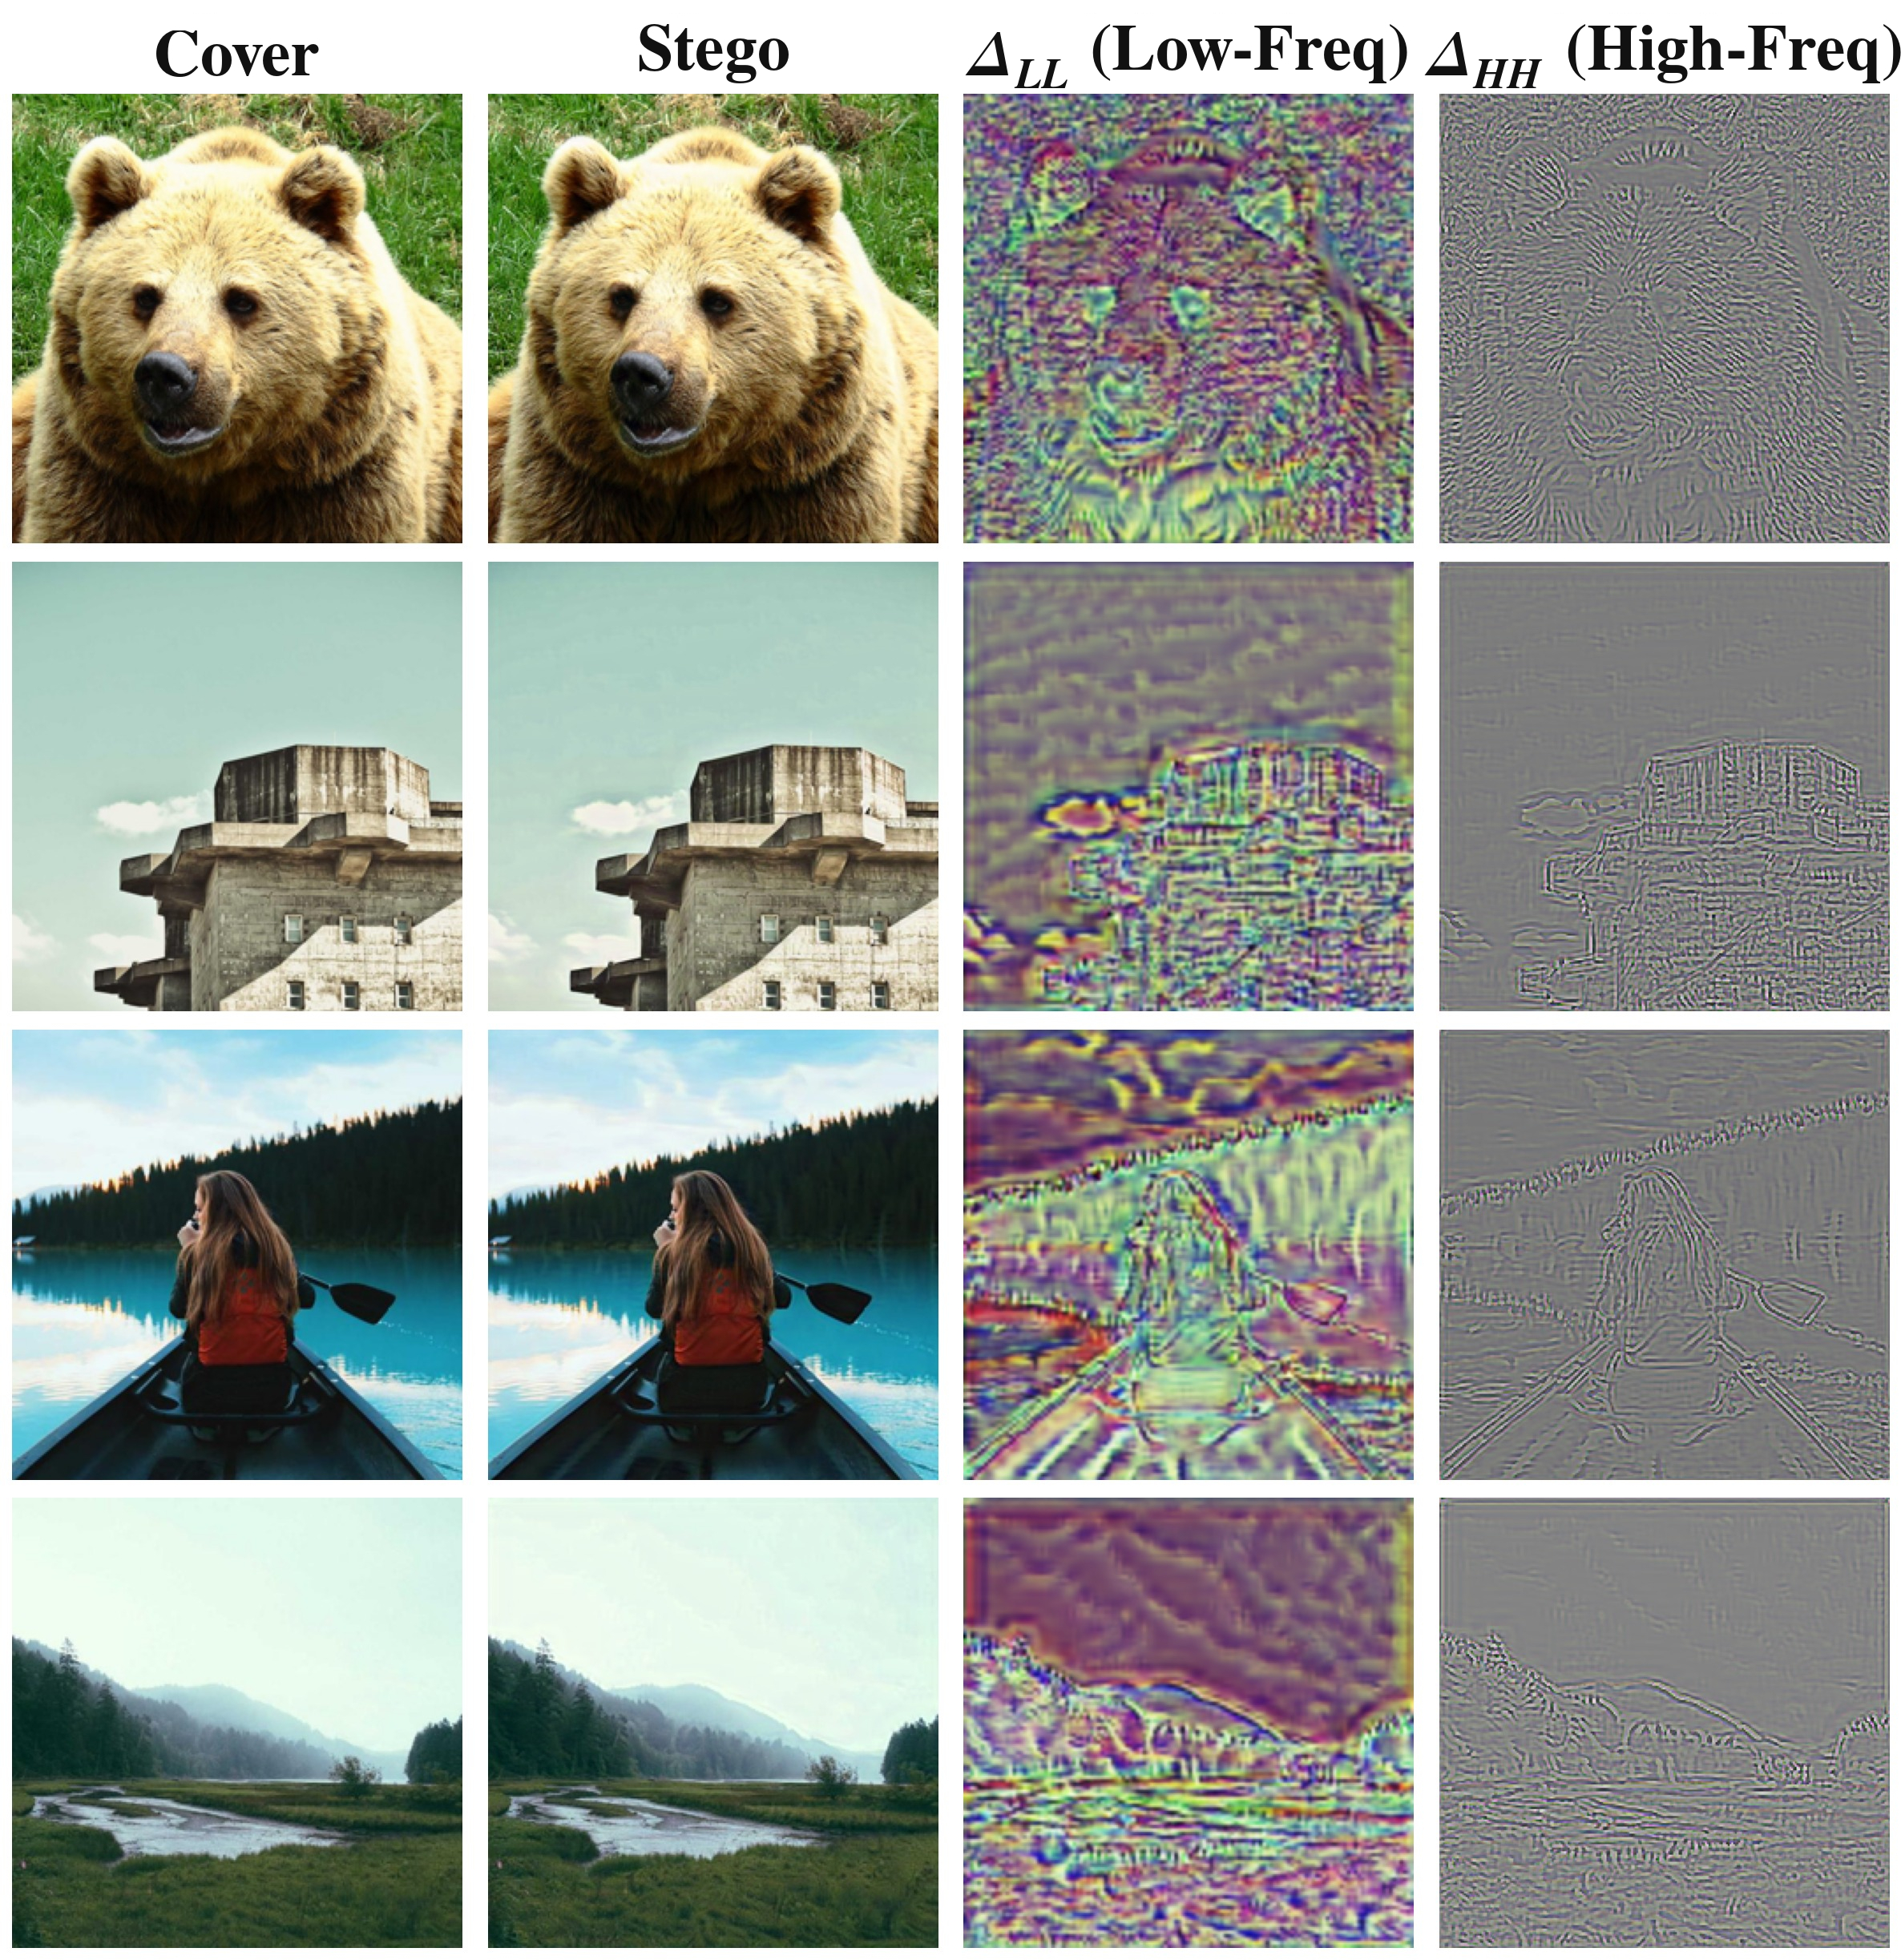
\includegraphics[width=\linewidth]{paper_assets/freq_decomp.jpg}
\par\smallskip\textbf{(a)}
\end{minipage}\hfill
\begin{minipage}[t]{0.485\textwidth}
\centering
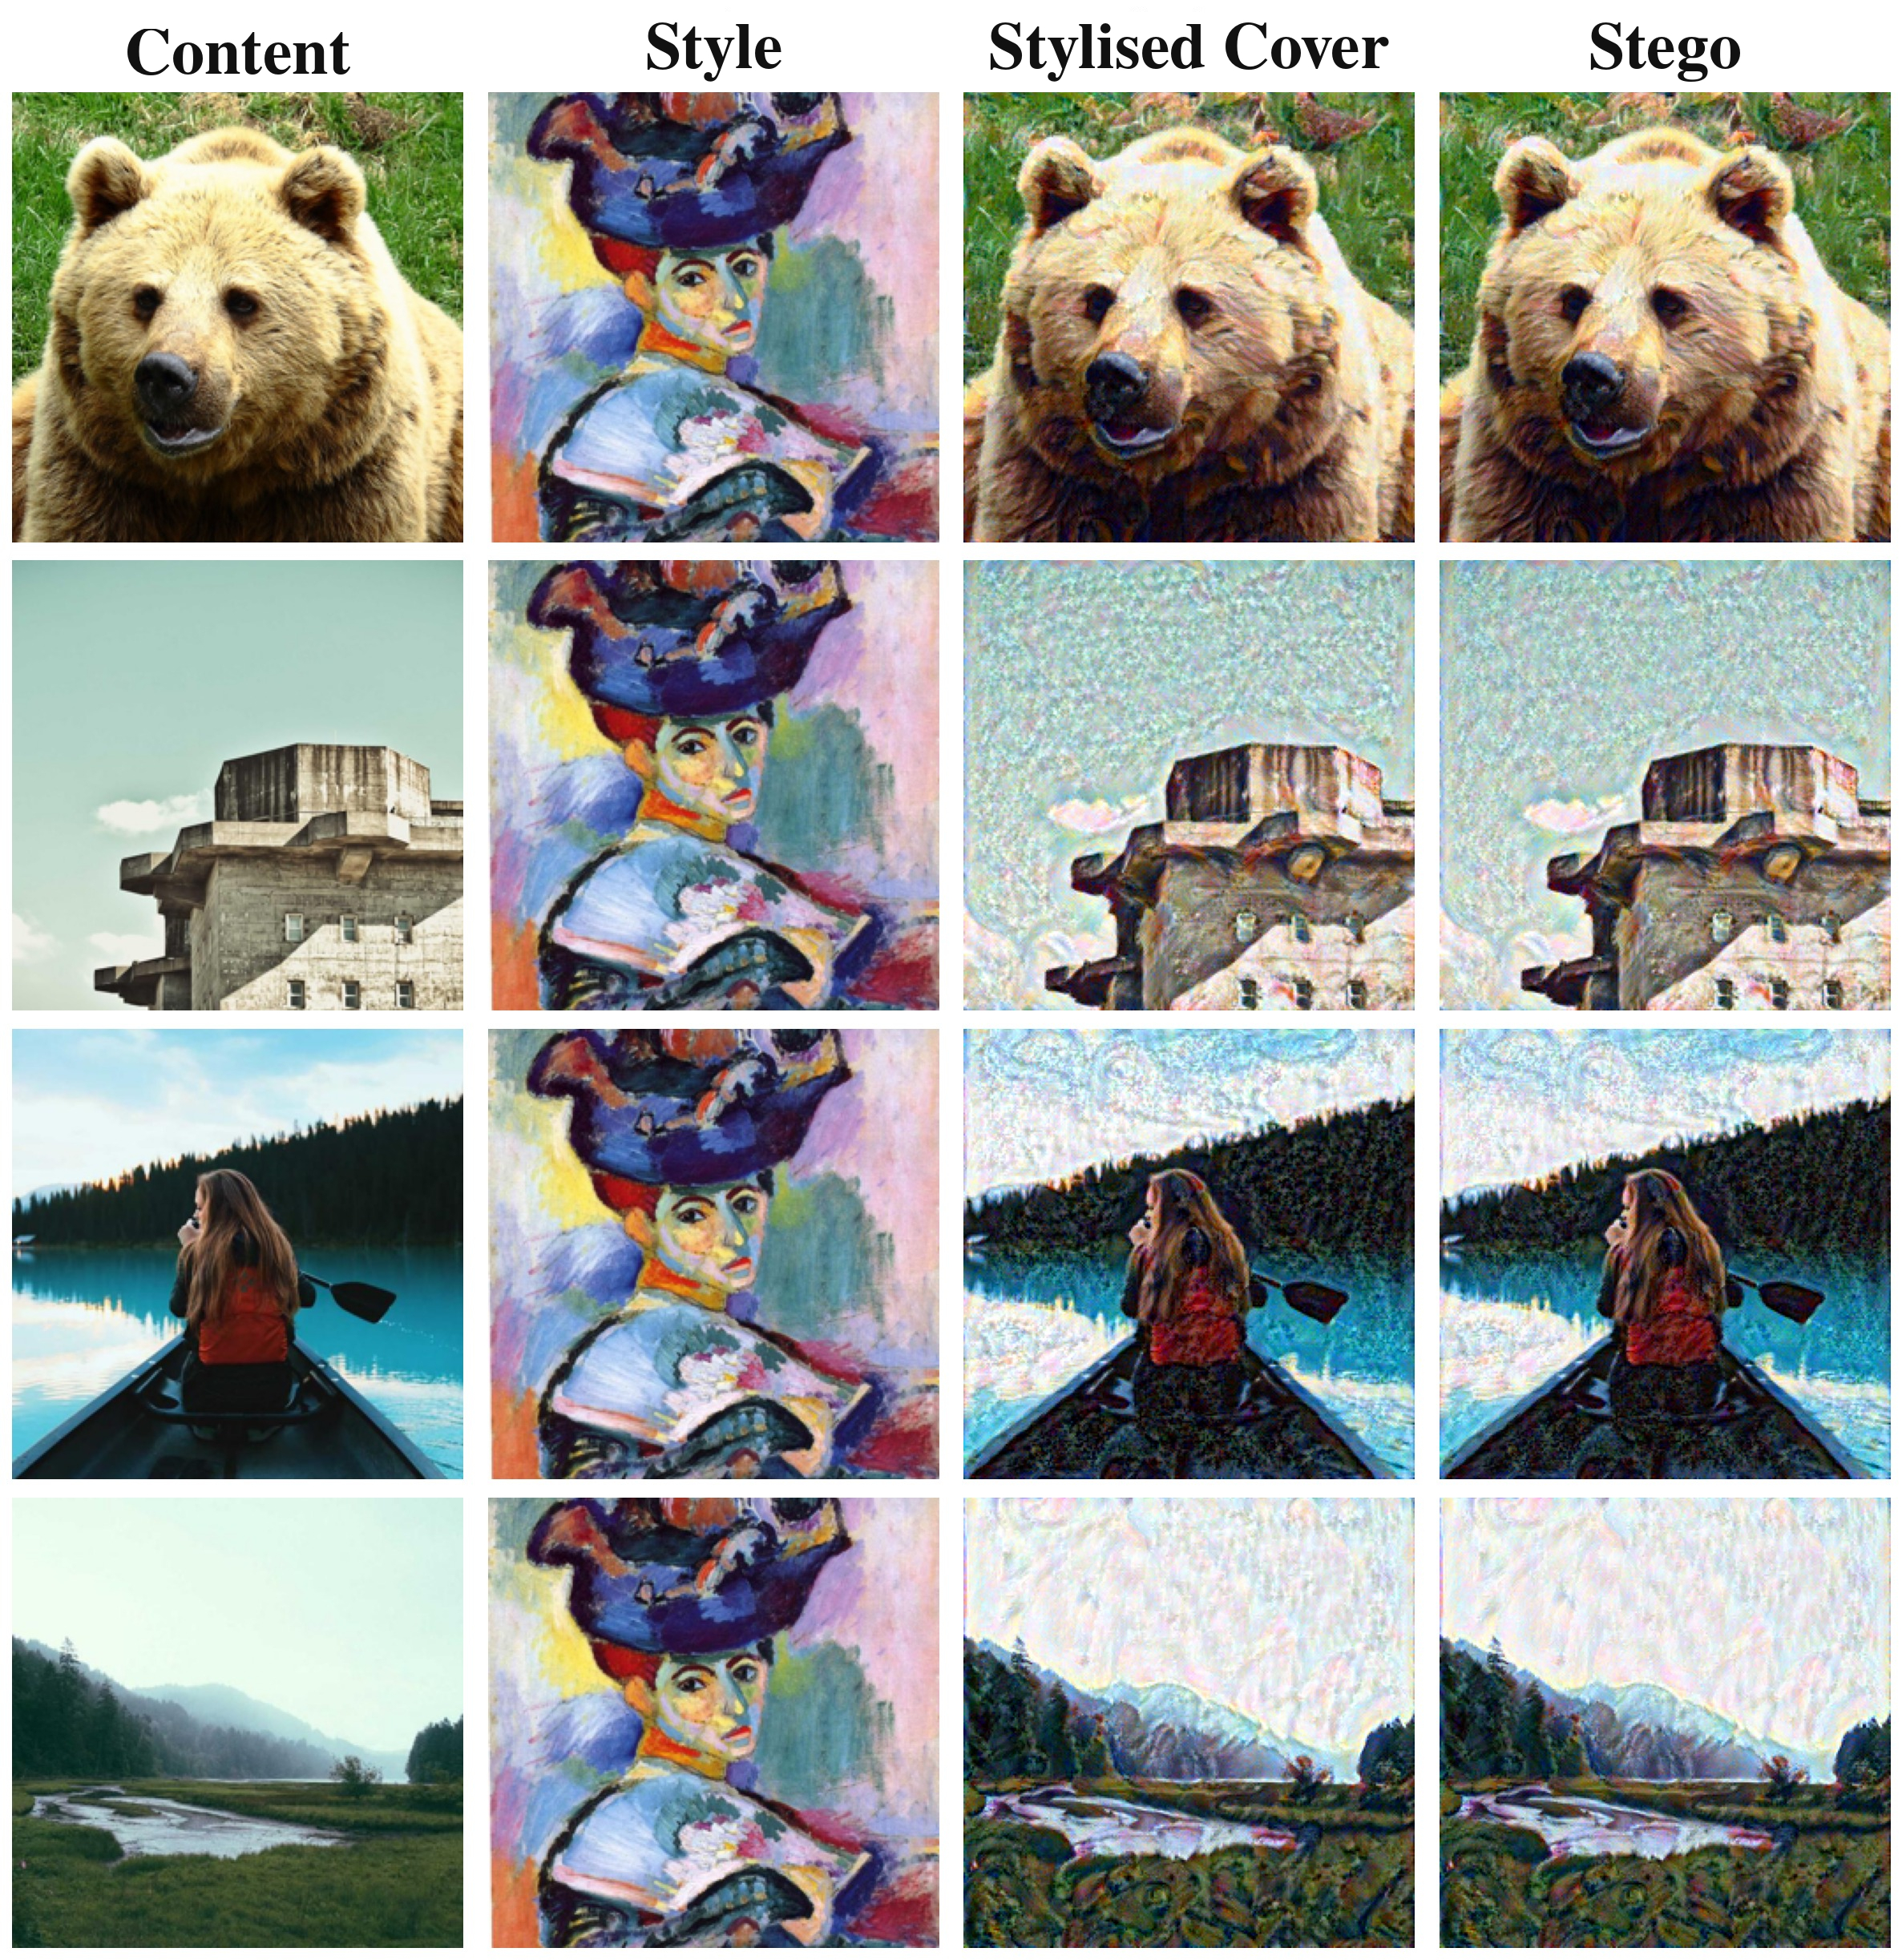
\includegraphics[width=\linewidth]{paper_assets/qualitative_grid.jpg}
\par\smallskip\textbf{(b)}
\end{minipage}
\caption{Qualitative inspection. (a) Residual decomposition into low- and high-frequency components; display contrast is enhanced for visibility. (b) Representative content, style, stylised-cover, and stego images from COCO, DIV2K, CelebA, and BOSSBase.}
\label{fig:freq_decomp}
\label{fig:qualitative}
\end{figure}

\revised{Table~\ref{tab:cross_dataset} acts as an out-of-distribution diagnostic stress check across four diverse domains (natural scenes, bicubic textures, facial structures, and sensor noise) with five images per dataset and one out-of-distribution style.} Mean PSNR ranges from $38.51$ to $38.82$\,dB. The sample is too small to support a broad generalisation claim, but it checks whether performance collapses outside the main COCO split.

\revised{Table~\ref{tab:robustness} evaluates real discrete cosine transform (DCT) JPEG compression (Quality 50) alongside standard filtering and geometric transformations from a separate extraction pipeline.} Within that pipeline, standard image-processing attacks change mean token MSE by at most $0.0015$. Serial rows are COCO-only and are therefore compared with the COCO Identity value rather than the four-dataset mean.

\begin{table}[t]
\centering
\begin{minipage}[t]{0.48\textwidth}
\centering
\scriptsize
\caption{Cross-dataset check with five images per dataset and one out-of-distribution style. MSE columns denote token MSE before and after the JPEG-style channel.}
\label{tab:cross_dataset}
\setlength{\tabcolsep}{4pt}
\begin{tabular}{lccc}
\toprule
\textbf{Dataset} & \textbf{PSNR} & \textbf{MSE} & \textbf{MSE(JP)} \\
\midrule
COCO     & 38.70 & 0.0136 & 0.0134 \\
DIV2K    & 38.71 & 0.0106 & 0.0105 \\
CelebA   & 38.51 & 0.0100 & 0.0099 \\
BOSSBase & 38.82 & 0.0101 & 0.0100 \\
\midrule
Avg & 38.68 & 0.0111 & 0.0110 \\
\bottomrule
\end{tabular}
\end{minipage}\hfill
\begin{minipage}[t]{0.48\textwidth}
\centering
\scriptsize
\caption{Representative robustness results from a separate extraction pipeline. Deltas for standard attacks use the four-dataset Identity mean; daggered serial rows use COCO Identity.}
\label{tab:robustness}
\setlength{\tabcolsep}{4pt}
\begin{tabular}{lcc}
\toprule
\textbf{Attack} & \textbf{Avg MSE} & \textbf{$\Delta$ (vs Id)} \\
\midrule
Identity       & $0.3602$ & --- \\
JPEG Q50       & $0.3598$ & $-0.0004$ \\
Gaussian $\sigma{=}0.05$ & $0.3600$ & $-0.0002$ \\
Resize 50\%    & $0.3600$ & $-0.0002$ \\
Median $3{\times}3$ & $0.3600$ & $-0.0002$ \\
Crop 80\%      & $0.3617$ & $+0.0015$ \\
\midrule
Serial-2$^{\dagger}$       & $0.3716$ & $-0.0019$ \\
Serial-3$^{\dagger}$       & $0.3706$ & $-0.0029$ \\
\bottomrule
\end{tabular}
\par\vspace{2pt}
{\footnotesize $^{\dagger}$Serial rows are measured on COCO only and use the COCO Identity value ($0.3735$).}
\end{minipage}
\end{table}

\subsection{Training Behaviour, Cost and Comparison Against Prior Art}
\label{sec:sota}
The archived validation score decreases from $5.68$ to $3.55$ over $41$ epochs, with intermediate fluctuations. Training takes approximately $870$\,s per epoch on the A100, or $9.9$ hours for the archived run. At $256\!\times\!256$ on an RTX~5070~Ti, the mean end-to-end time is $0.0223$\,s per image: $0.0023$\,s for the tokenizer, $0.0073$\,s for the stego encoder, $0.0004$\,s for the stego decoder, and $0.0124$\,s for the reverse decoder. On one CPU thread at $192\!\times\!192$, the stego encoder and decoder take $0.0690$ and $0.0051$\,s, respectively. The model contains $0.94$\,M tokenizer, $0.98$\,M encoder, $0.82$\,M stego-decoder, and $7.93$\,M reverse-decoder parameters ($10.7$\,M total, excluding frozen VGG-19). The embedding path uses the first two modules.

Figure~\ref{fig:training} shows the archived validation trajectory and component losses across the three scheduled phases.

\begin{figure}[!t]
\centering
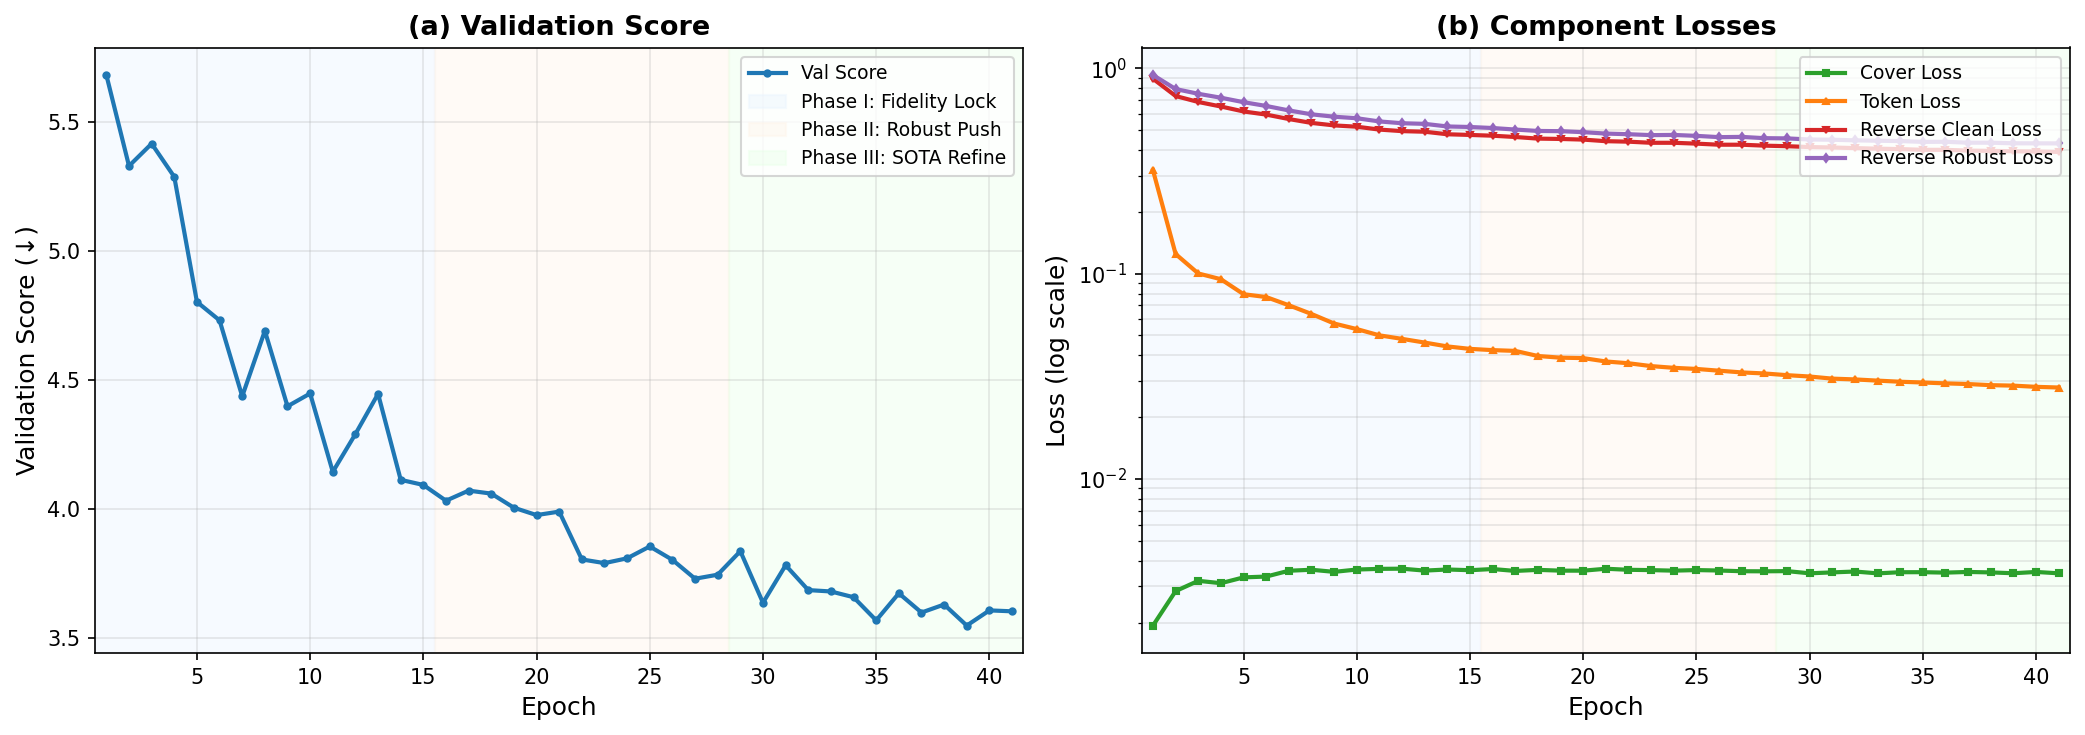
\includegraphics[width=0.96\textwidth]{paper_assets/training_curve.png}
\caption{Validation score and component losses over the archived 41-epoch run. Shading marks the three training phases.}
\label{fig:training}
\end{figure}

\revised{Table~\ref{tab:sota_style} provides a bibliographic taxonomy characterizing published style-transfer hiding formulations rather than a competitive ranking, as metric targets differ fundamentally across paradigms: Quaternion-Style~\cite{quat2021} measures fidelity against the pre-style cover, IHST~\cite{ihst2024} evaluates recovered secret fidelity, and FGSS evaluates stego distortion against the stylized carrier $\mathbf{X}_{\text{cover}}$. Matched evaluation against the direct inverse baseline is established in Table~\ref{tab:reverse_and_serial}.} Other style-transfer methods~\cite{sstegogan2024,sddpm2025,stisgan2026} are discussed in Section~\ref{sec:relwork}.

\begin{table}[htbp]
\centering
\scriptsize
\caption{Reported metrics for selected style-transfer hiding methods. Metric targets differ across rows, so the values are not directly comparable.}
\label{tab:sota_style}
\setlength{\tabcolsep}{8pt}
\small
\begin{tabular}{lcccc}
\toprule
\textbf{Method} & \textbf{Year} & \textbf{PSNR$\uparrow$} & \textbf{SSIM$\uparrow$} & \textbf{Rev.} \\
\midrule
Self-Contained~\cite{wacv2020}     & 2020 & ---       & ---        & \checkmark \\
Quaternion~\cite{quat2021}         & 2021 & \textbf{42.30}   & $0.987$    & --- \\
IHST~\cite{ihst2024}               & 2024 & $35.90$   & $0.960$    & \checkmark \\
\midrule
Ours                       & 2026 & $39.61$ & \textbf{0.991} & \textbf{0.81} \\
\bottomrule
\end{tabular}
\par\vspace{4pt}
{\footnotesize Metric target: Self-Contained reports L2/SSIM/LPIPS with no PSNR; Quaternion measures stego~$\leftrightarrow$~\emph{pre-style} cover; IHST measures recovered~$\leftrightarrow$~secret (not cover fidelity); Ours measures stego~$\leftrightarrow$~\emph{styled} cover.}
\end{table}

\subsection{Discussion and Limitations}
Four components define the method: the target-derived threshold calibrates the cover penalty, the frequency term discourages low-frequency residual energy, the semantic token reduces spatial payload, and the reverse/serial losses train recovery after repeated transformations.

\revised{High cover fidelity alone does not ensure cryptographic security. Grouped five-fold cross-validation on $600$ cover/stego pairs gives ROC-AUC $0.848$ for a full Spatial Rich Model~\cite{srm}, $0.905$ for a locally trained XuNet-like probe~\cite{xunet}, and $0.779$ for an SRNet-tiny probe~\cite{srnet}. These above-chance detection rates stem from the fact that neural style transfer alters spatial feature statistics while residual embedding introduces subtle micro-texture perturbations detectable by high-pass filter banks. FGSS is explicitly positioned as perceptual/functional steganography for self-contained image distribution and serial stylisation survival, rather than zero-detectability against an informed warden. Integrating adversarial steganalysis objectives and scaling to arbitrary styles via feed-forward diffusion priors remain key future goals.}

\section{Conclusion}
% SOURCE: run_summary.json, paper_table_main.csv, robustness_metrics.csv
FGSS represents the secret with a $64\!\times\!32\!\times\!32$ semantic token and thumbnail. A target-derived MSE threshold calibrates a soft cover penalty, while a wavelet-inspired term discourages low-frequency residual energy. Oracle-guided reverse decoding and future-pass supervision support recovery after repeated stylisation.

On $600$ COCO val2017 pairs, FGSS obtains $39.61$\,dB cover PSNR and $0.9914$ SSIM. Clean-channel reverse SSIM increases from $0.5234$ to $0.8070$; the oracle-token diagnostic reaches $0.8136$. A five-image-per-dataset check gives $38.51$--$38.82$\,dB on four datasets, and a separate robustness pipeline shows standard-attack token-MSE changes no larger than $0.0015$. In the reduced single-pair ablation, enabling the target-calibrated penalty changes cover PSNR by $5.76$\,dB. The $1.9$\,M-parameter embedding path runs in under $0.01$\,s on the measured GPU. The above-chance steganalysis results remain the main limitation.

\section*{Acknowledgements}
The authors thank Tra Vinh University and Tien Giang University for their general support. We acknowledge time and facility support from Tra Vinh University.

\begin{thebibliography}{99}
\bibitem{isn} Lu, S.-P., Wang, R., Zhong, T., Rosin, P.L.: Large-capacity image steganography based on invertible neural networks. In: CVPR, pp. 10816--10825 (2021)
\bibitem{riis} Xu, Y., Mou, C., Hu, Y., Xie, J., Zhang, J.: Robust invertible image steganography. In: CVPR, pp. 7875--7884 (2022)
\bibitem{rmsteg} Ye, H., Zhang, S., Jiang, S., Liao, J., Gu, S., Zheng, D., Wang, C., Li, C.: Robust message embedding via attention flow-based steganography. In: CVPR, pp. 12840--12849 (2025)
\bibitem{wacv2020} Chen, H.-Y., Fang, I.-S., Cheng, C.-M., Chiu, W.-C.: Self-contained stylization via steganography for reverse and serial style transfer. In: WACV, pp. 2163--2171 (2020)
\bibitem{stylestegan2023} Liang, X., Liu, B., Ying, Q., Qian, Z., Cho, H., Zhang, X.: StyleStegan: leak-free style transfer based on feature steganography. In: APSIPA ASC, pp. 1443--1450 (2023). \doi{10.1109/APSIPAASC58517.2023.10317570}
\bibitem{sstegogan2024} Li, L., Zhang, X., Chen, K., Feng, G., Wu, D., Zhang, W.: Image steganography and style transformation based on generative adversarial network. Mathematics \textbf{12}(4), 615 (2024). \doi{10.3390/math12040615}
\bibitem{sst2024} Shi, R., Wang, Z., Hao, Y., Zhang, X.: Steganography in style transfer. IEEE Trans. Artif. Intell. \textbf{5}(12), 6054--6065 (2024). \doi{10.1109/TAI.2024.3379946}
\bibitem{ihst2024} Zhang, F., Feng, B., Xia, Z., Weng, J., Lu, W., Chen, B.: Conditional image hiding network based on style transfer. Inf. Sci. \textbf{662}, 120225 (2024). \doi{10.1016/j.ins.2024.120225}
\bibitem{css2024} Zhang, X., Zhang, M., Wang, X., Huang, S., Di, F.: Constructive robust steganography algorithm based on style transfer. CMC \textbf{81}(1), 1433--1448 (2024). \doi{10.32604/cmc.2024.056742}
\bibitem{sddpm2025} Lin, Y.-H., Huang, C.-P., Huang, P.-S.: A steganographic message transmission method based on style transfer and DDPM. Electronics \textbf{14}(16), 3258 (2025). \doi{10.3390/electronics14163258}
\bibitem{stisgan2026} Luo, Y., Chen, Z., Lu, B., Huang, Y., Fu, Q., Qin, S., Liu, J.: Style transfer image steganography based on GANs with frequency domain attention and autoencoder networks. Appl. Soft Comput. \textbf{188}, 114440 (2026). \doi{10.1016/j.asoc.2025.114440}
\bibitem{coco} Lin, T.-Y., Maire, M., Belongie, S., Hays, J., Perona, P., Ramanan, D., Doll\'ar, P., Zitnick, C.L.: Microsoft COCO: common objects in context. In: ECCV. LNCS, vol. 8693, pp. 740--755 (2014). \doi{10.1007/978-3-319-10602-1_48}
\bibitem{ssim} Wang, Z., Bovik, A.C., Sheikh, H.R., Simoncelli, E.P.: Image quality assessment: from error visibility to structural similarity. IEEE TIP \textbf{13}(4), 600--612 (2004). \doi{10.1109/TIP.2003.819861}
\bibitem{lpips} Zhang, R., Isola, P., Efros, A.A., Shechtman, E., Wang, O.: The unreasonable effectiveness of deep features as a perceptual metric. In: CVPR, pp. 586--595 (2018)
\bibitem{rfs2023} Lan, Y., Shang, F., Yang, J., Kang, X., Li, E.: Robust image steganography: hiding messages in frequency coefficients. Proc. AAAI Conf. Artif. Intell. \textbf{37}(12), 14955--14963 (2023). \doi{10.1609/aaai.v37i12.26746}
\bibitem{srnet} Boroumand, M., Chen, M., Fridrich, J.: Deep residual network for steganalysis of digital images. IEEE TIFS \textbf{14}(5), 1181--1193 (2019). \doi{10.1109/TIFS.2018.2871749}
\bibitem{xunet} Xu, G., Wu, H.-Z., Shi, Y.-Q.: Structural design of convolutional neural networks for steganalysis. IEEE SPL \textbf{23}(5), 708--712 (2016). \doi{10.1109/LSP.2016.2548421}
\bibitem{ideas2022} Liu, X., Ma, Z., Ma, J., Zhang, J., Schaefer, G., Fang, H.: Image disentanglement autoencoder for steganography without embedding. In: CVPR, pp. 2303--2312 (2022)
\bibitem{siswe2023} Ma, Z., Zhu, Y., Luo, G., Liu, X., Schaefer, G., Fang, H.: Robust steganography without embedding based on secure container synthesis and iterative message recovery. In: IJCAI, pp. 4838--4846 (2023). \doi{10.24963/ijcai.2023/538}
\bibitem{cross} Yu, J., Zhang, X., Xu, Y., Zhang, J.: CRoSS: diffusion model makes controllable, robust and secure image steganography. Adv. Neural Inf. Process. Syst. \textbf{36}, 80730--80743 (2023). \doi{10.52202/075280-3539}
\bibitem{quat2021} Li, Q., Wang, X., Ma, B., Wang, X., Wang, C., Xia, Z., Shi, Y.: Image steganography based on style transfer and quaternion exponent moments. Appl. Soft Comput. \textbf{110}, 107618 (2021). \doi{10.1016/j.asoc.2021.107618}
\bibitem{gatys} Gatys, L.A., Ecker, A.S., Bethge, M.: Image style transfer using convolutional neural networks. In: CVPR, pp. 2414--2423 (2016)
\bibitem{adam} Kingma, D.P., Ba, J.: Adam: a method for stochastic optimization. In: ICLR (2015)
\bibitem{vgg} Simonyan, K., Zisserman, A.: Very deep convolutional networks for large-scale image recognition. In: ICLR (2015)
\bibitem{gelu} Hendrycks, D., Gimpel, K.: Gaussian error linear units (GELUs). arXiv:1606.08415 (2016)
\bibitem{adain} Huang, X., Belongie, S.: Arbitrary style transfer in real-time with adaptive instance normalization. In: ICCV, pp. 1501--1510 (2017)
\bibitem{srm} Fridrich, J., Kodovsk\'y, J.: Rich models for steganalysis of digital images. IEEE TIFS \textbf{7}(3), 868--882 (2012). \doi{10.1109/TIFS.2012.2190402}
\end{thebibliography}

\end{document}
